%\documentclass[journal]{IEEEtran}
\documentclass[12pt, draftcls, onecolumn]{IEEEtran}
\makeatletter
% journal (default) and conference
\def\subsubsection{\@startsection{subsubsection}% name
                                 {3}% level
                                 {\z@}% indent (formerly \parindent)
                                 {0ex plus 0.1ex minus 0.1ex}% before skip
                                 {0ex}% after skip
                                 {\normalfont\normalsize\bfseries}}% style
\makeatother
\usepackage[T1]{fontenc}% optional T1 font encoding
%\usepackage{graphicx}
\usepackage{subfigure}
\usepackage{ulem}
\usepackage{amsmath}
\allowdisplaybreaks
\usepackage{hhline}
\usepackage{yfonts,color}
\usepackage{soul,xcolor}
\usepackage{verbatim}
\usepackage{amsmath}
\allowdisplaybreaks
\usepackage{amssymb}
\usepackage{amsthm}
\usepackage{float}
\usepackage{bm}
\usepackage{url}
\usepackage{array}
\usepackage{cite}
\usepackage{graphicx}
\usepackage{framed} % for frame
\usepackage{balance} % balance
\usepackage{epsfig,epstopdf}
\usepackage{booktabs}
\usepackage{courier}
\usepackage{subfigure}
\usepackage{enumerate}
\usepackage[options]{algorithm2e}
\usepackage{algorithm}
\usepackage[export]{adjustbox}
\newtheorem{definition}{Definition}
\newtheorem{theorem}{Theorem}
\newtheorem{lemma}[theorem]{Lemma}
\newtheorem{proposition}[theorem]{Proposition}
%\newtheorem{proposition}{Proposition}
\newtheorem{corollary}[theorem]{Corollary}
\newtheorem{assumption}{Assumption}
\newtheorem{remark}{Remark}
\newcommand{\rom}[1]{\uppercase\expandafter{\romannumeral #1\relax}}
\usepackage{color}
\usepackage{soul,xcolor}
\newcommand{\nm}[1]{{\color{blue}\text{\bf{[NM: #1]}}}}
\newcommand{\sst}[1]{\st{#1}}
\newcommand{\gs}[1]{{\color{orange}\bf{[GS: #1]}}}
\newcommand{\remove}[1]{{\color{magenta}{\bf REMOVE: [#1]}}}
%\newcommand{\nm}[1]{}
%\newcommand{\sst}[1]{}
%\newcommand{\gs}[1]{}
%\newcommand{\remove}[1]{}
\newcommand{\add}[1]{{\color{red}{#1}}}
\newcommand{\ull}[1]{\textbf{\color{red}\ul{#1}}}
%\pagestyle{empty}
\normalem
\begin{document} 
\setulcolor{red}
\setul{red}{2pt}
\title{ECE64700: Homework III}
\author{Bharath Keshavamurthy}
\maketitle
\section{Projection Gradient Descent: Simulation Assignment}
\subsection{Theory of Optimality}
\[minimize\ x_1^2 + 9x_2^2\]
\[subject\ to\ 2x_1 + x_2 \geq 1,\ x_1 + 3x_2 \geq 1,\ x_1 \geq 0,\ x_2 \geq 0\]
This is a \textbf{Convex Optimization Problem} because the objective function is convex and the feasible set is an intersection of a finite number of halfspaces, i.e. a polyhedron.
\\Formulate the Lagrangian as follows,
\[\mathcal{L}(x_1,\ x_2,\ \lambda_1,\ \lambda_2)\ =\ x_1^2 + 9x_2^2 + \lambda_1(1 - 2x_1 - x_2) + \lambda_2(1 - x_1 - 3x_2)\]
\[\mathcal{L}(x_1,\ x_2,\ \lambda_1,\ \lambda_2)\ =\ x_1^2 + 9x_2^2 - (2\lambda_1 + \lambda_2)x_1 - (\lambda_1 + 3\lambda_2)x_2 + \lambda_1 + \lambda_2\]
\[g(\lambda_1,\ \lambda_2)\ =\ min_{x_1,\ x_2}\ \mathcal{L}(x_1,\ x_2,\ \lambda_1,\ \lambda_2)\]
Solving,
\[\frac{\partial \mathcal{L}}{\partial x_1}\ =\ 0\]
\[2x_1 - 2\lambda_1 - \lambda_2\ =\ 0\]
\[x_1\ =\ \frac{2\lambda_1 + \lambda_2}{2}\]
\[\frac{\partial \mathcal{L}}{\partial x_2}\ =\ 0\]
\[-\lambda_1 - 3\lambda_2 + 18x_2\ =\ 0\]
\[x_2\ =\ \frac{\lambda_1 + 3\lambda_2}{18}\]
\[g(\lambda_1,\ \lambda_2)\ =\ (\frac{2\lambda_1 + \lambda_2}{2})^2 + 9(\frac{\lambda_1 + 3\lambda_2}{18})^2 - \frac{(2\lambda_1 + \lambda_2)^2}{2} - \frac{(\lambda_1 + 3\lambda_2)^2}{18} + \lambda_1 + \lambda_2\]
\[g(\lambda_1,\ \lambda_2)\ =\ -\frac{(2\lambda_1 + \lambda_2)^2}{4} - \frac{(\lambda_1 + 3\lambda_2)^2}{36} + \lambda_1 + \lambda_2\]
\clearpage
\[\lambda_1^*,\ \lambda_2^*\ =\ max_{\lambda_1,\ \lambda_2}\ g(\lambda_1,\ \lambda_2)\]
\[subject\ to\ \lambda_1 \geq 0,\ \lambda_2 \geq 0\]
Solving,
\[\frac{\partial g}{\partial \lambda_1}\ =\ 0\]
\[-2\lambda_1 - \lambda_2 - \frac{\lambda_1 + 3\lambda_2}{18} + 1\ =\ 0\]
\[37\lambda_1 + 21\lambda_2 - 18\ =\ 0\]
\[\frac{\partial g}{\partial \lambda_2}\ =\ 0\]
\[-\frac{2\lambda_1 + \lambda_2}{2} - \frac{\lambda_1 + 3\lambda_2}{6} + 1\ =\ 0\]
\[7\lambda_1 + 6\lambda_2 - 6\ =\ 0\]
Solving the two equations for two unknowns, we get,
\[\lambda_1\ =\ -\frac{6}{25} < 0 \longrightarrow\ violates\ constraints\]
\[\lambda_2\ =\ \frac{32}{25}\]
Let's try with $\lambda_1\ =\ 0$. Then,
\[\lambda_2\ =\ 1\]
Now, we make the following statements:
\begin{itemize}
    \item $\lambda_1^*\ =\ 0\ and\ \lambda_2^*\ =\ 1$ satisfy the \textbf{Dual Feasibility Constraints}
    \item Using $\lambda_1^*\ =\ 0\ and\ \lambda_2^*\ =\ 1$,
    \[x_1^*\ =\ \frac{1}{2}\ and\ x_2^*\ =\ \frac{1}{6}\]
    These values satisfy the \textbf{Primal Feasibility Constraints}, i.e. 
    \[2x_1^* + x_2^* \geq 1\]
    \[x_1^* + 3x_2^* \geq 1\]
    \[x_1^* \geq 0\]
    \[x_2^* \geq 0\]
    \item The \textbf{Complementary Slackness} condition is satisfied, i.e.
    \[\lambda_1 f_1(x_1^*,\ x_2^*)\ =\ 0\], because $\lambda_1\ =\ 0$ while $f_1(x_1^*,\ x_2^*)\ =\ \frac{7}{6}$
    \[\lambda_2 f_2(x_1^*,\ x_2^*)\ =\ 0\], because $f_2(x_1^*,\ x_2^*)\ =\ 0$ while $\lambda_2\ =\ 1$
    \item $(x_1^*,\ x_2^*)$ is the minimizer of the Lagrangian over all $\vec{x}$.
    \\Mathematically,
    \[\triangledown f_0(x_1^*,\ x_2^*) + \lambda_1^* \triangledown f_1(x_1^*,\ x_2^*) + \lambda_2^* \triangledown f_2(x_1^*,\ x_2^*)\ =\ 0\]
\end{itemize}
Based on the points mentioned above, the solution obtained satisfies the \textbf{KKT Conditions} and hence the \textbf{duality gap is zero} which implies the following,
\[f_0(x_1^*,\ x_2^*)\ =\ \mathcal{L}(x_1^*,\ x_2^*,\ \lambda_1^*,\ \lambda_2^*)\ =\ g(\lambda_1^*,\ \lambda_2^*)\ =\ \frac{1}{2}\]
\textbf{The simulation should yield the same results}.
\subsection{Simulation: Pseudo code}
\begin{algorithm}[H]
\SetAlgoLined
\KwResult{Solution - $(x_1^*,\ x_2^*)\ =\ (\frac{1}{2},\ \frac{1}{6})$ with $f_0(x_1^*,\ x_2^*)\ =\ \frac{1}{2}$}
 \textbf{Initialization}: Pick an initial point $\vec{x}_0 \in \mathcal{F}$\;
 \\Pick a step-size, $\gamma\ =\ 0.1$\newline
 \While{$\vec{x}_{k+1}\ !=\ [\vec{x}_k - \gamma \triangledown f_0(\vec{x}_k)]^+$}{
  $\vec{x}_{k+1}\ =\ [\vec{x}_k - \gamma \triangledown f_0(\vec{x}_k)]^+$;
 }
\caption{Projection Gradient Descent Algorithm}
\end{algorithm}
Here, the $[\vec{x}]^+$ operation refers to the projection algorithm which is implemented in Python using the \textbf{Vector Projection Logic} described below.
The component of a vector $\vec{a}$ along another vector $\vec{b}$ is given by,
\[a_1\ =\ \frac{\vec{a} \cdot \vec{b}}{||\vec{b}||}\]
The projection of $\vec{a}$ along $\vec{b}$ is then given by,
\[\vec{a}_1\ =\ a_1 \frac{\vec{b}}{||\vec{b}||}\]
Taking the collection of hyperplanes constituting the boundary of the feasible set, i.e.,
\[\{\{(0, \infty), (0, 1)\}, \{(0, 1), (0.4, 0.2)\}, \{(0.4, 0.2), (1, 0)]\}, \{(1, 0), (\infty, 0)\}\},\]
We find the \textit{<smallest\_distance, closest\_point>} pair for the out-of-bounds point with respect to each of these hyperplanes and then find the smallest distance among them. The point corresponding to the smallest distance among all four hyperplanes is the projection of the out-of-bounds point.
\\Please refer to the source code (\textit{ProjectionGradientDescent.py}) for further details.
\subsection{Simulation: Results}
\begin{figure}[t]
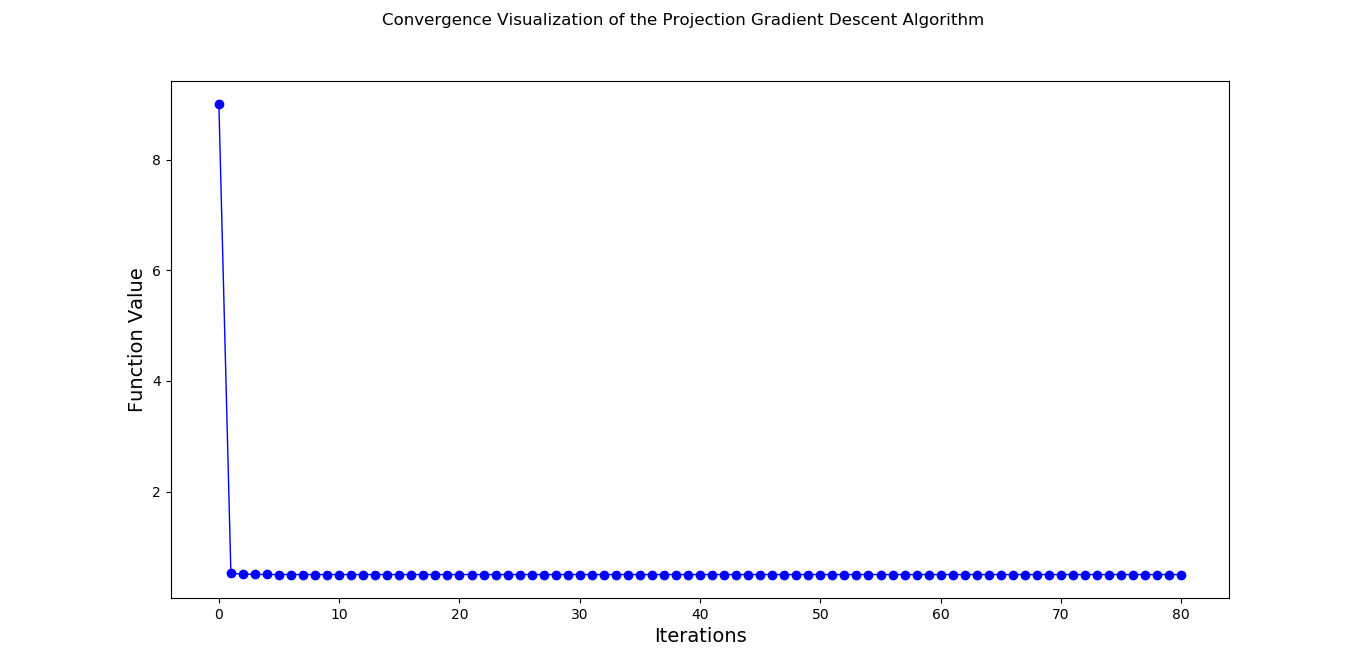
\includegraphics[width=1.0\textwidth]{PGD_Convergence_Gamma_Point1.png}
\caption{Convergence Visualization of the Projection Gradient Descent Algorithm with step size $0.1$}
\label{fig:mesh1}
\centering
\end{figure}
\begin{figure}[t]
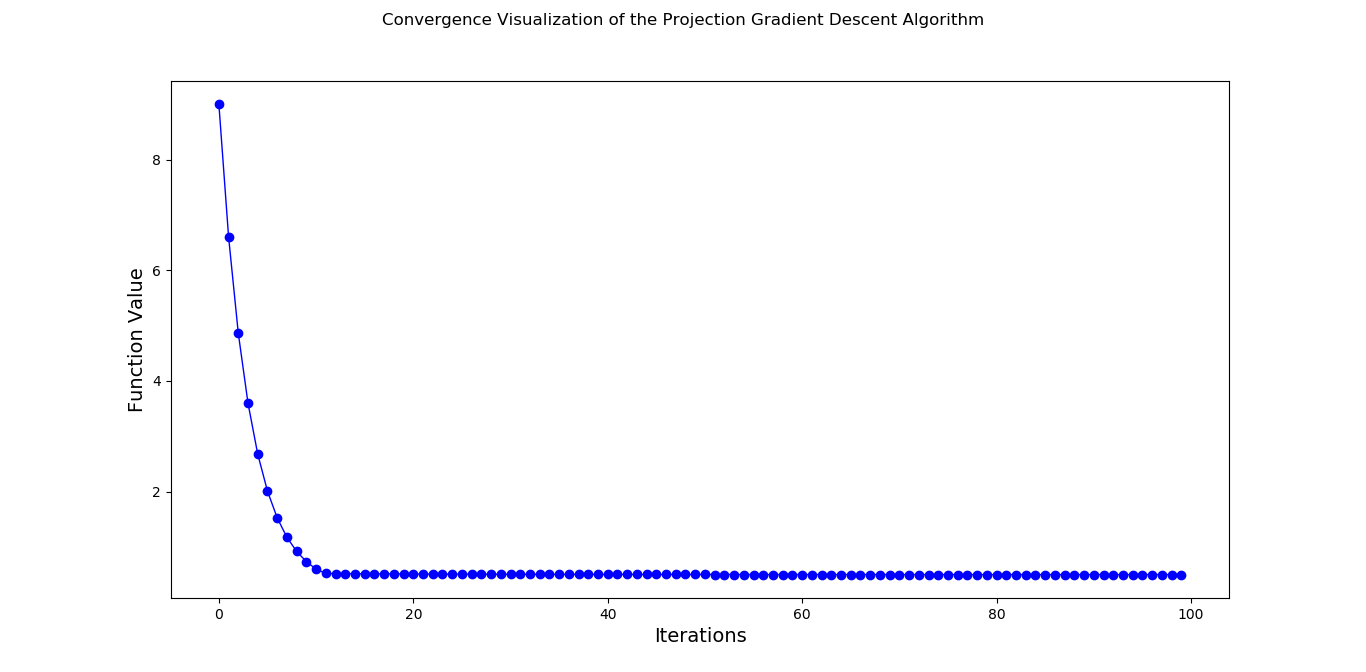
\includegraphics[width=1.0\textwidth]{PGD_Convergence_Gamma_Point01.png}
\caption{Convergence Visualization of the Projection Gradient Descent Algorithm with step size $0.01$}
\label{fig:mesh2}
\centering
\end{figure}
\begin{figure}[t]
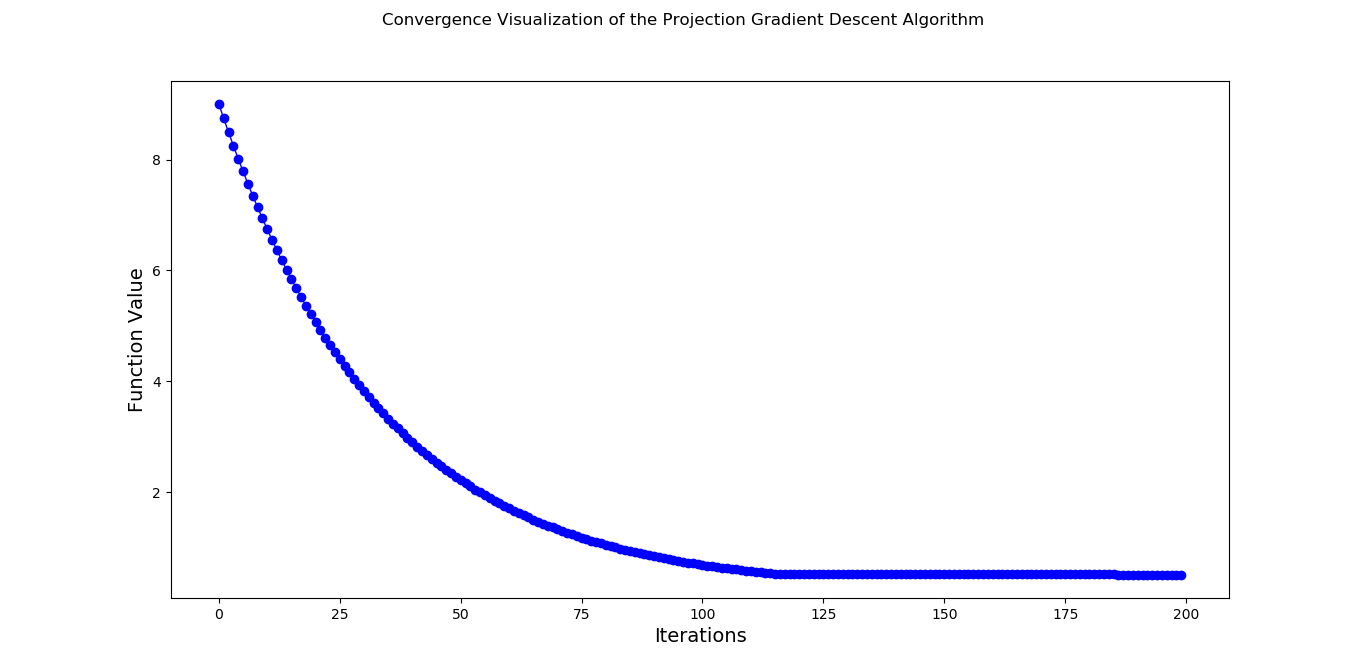
\includegraphics[width=1.0\textwidth]{PGD_Convergence_Gamma_Point001.png}
\caption{Convergence Visualization of the Projection Gradient Descent Algorithm with step size $0.001$}
\label{fig:mesh3}
\centering
\end{figure}
\begin{figure}[t]
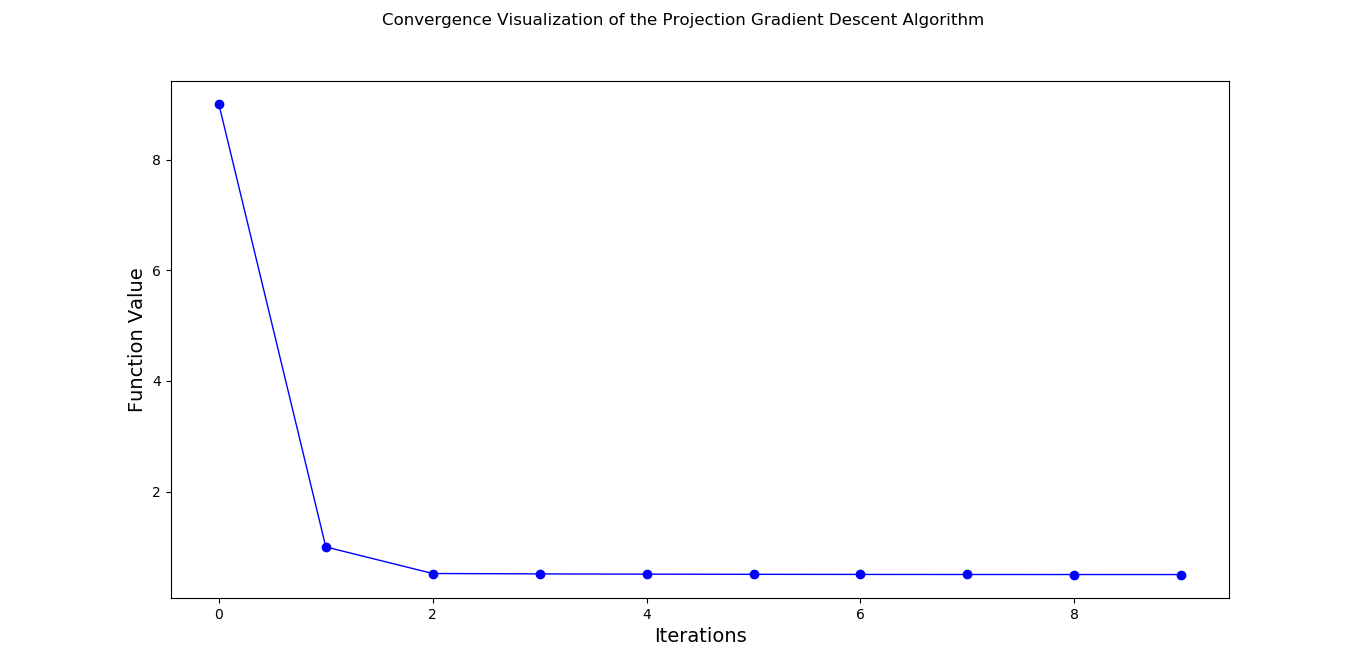
\includegraphics[width=1.0\textwidth]{PGD_Convergence_Gamma_Point5.png}
\caption{Convergence Visualization of the Projection Gradient Descent Algorithm with step size $0.5$}
\label{fig:mesh4}
\centering
\end{figure}
\begin{figure}[t]
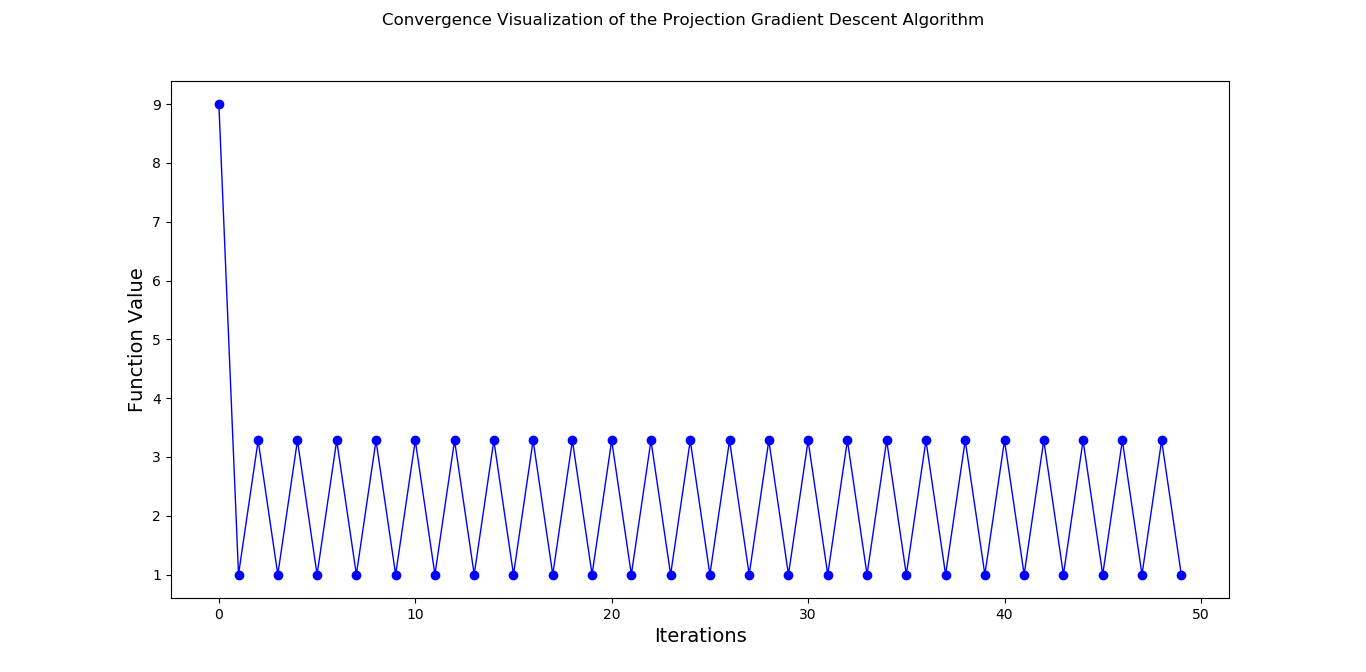
\includegraphics[width=1.0\textwidth]{PGD_Convergence_Gamma_1.png}
\caption{Convergence Visualization of the Projection Gradient Descent Algorithm with step size $1$}
\label{fig:mesh5}
\centering
\end{figure}
\begin{figure}[t]
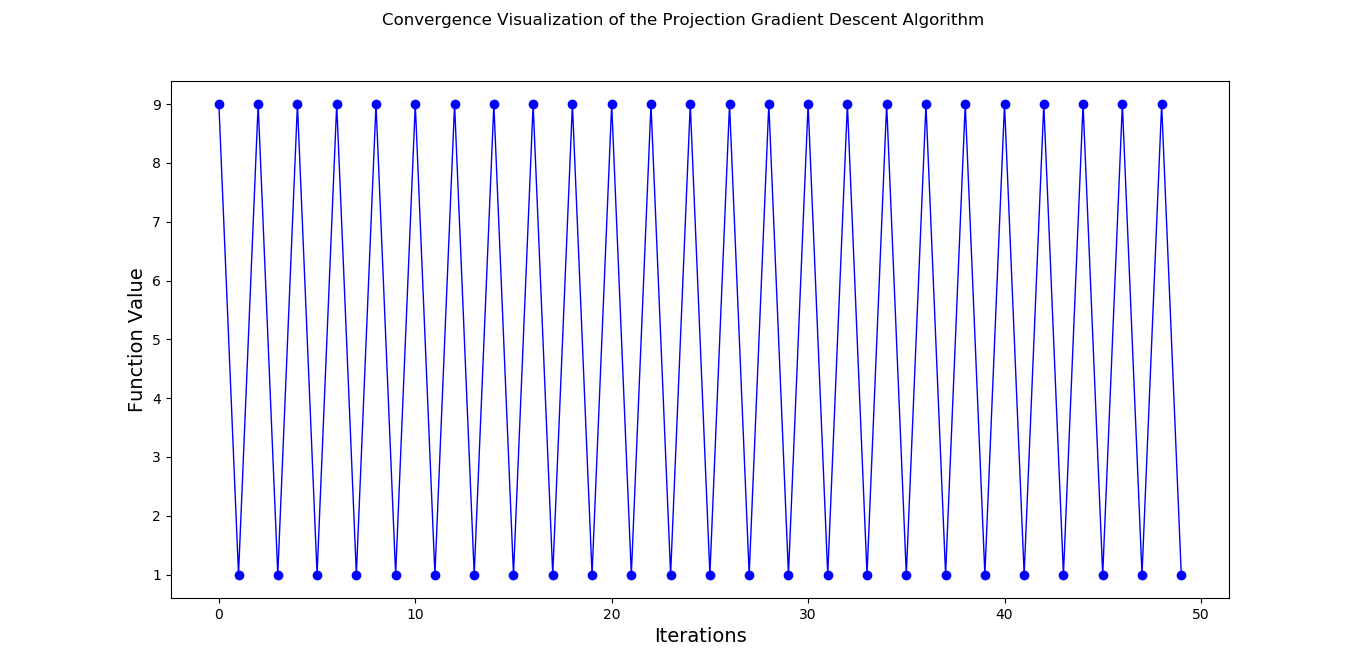
\includegraphics[width=1.0\textwidth]{PGD_Convergence_Gamma_10.png}
\caption{Convergence Visualization of the Projection Gradient Descent Algorithm with step size $10$}
\label{fig:mesh6}
\centering
\end{figure}
\begin{figure}[t]
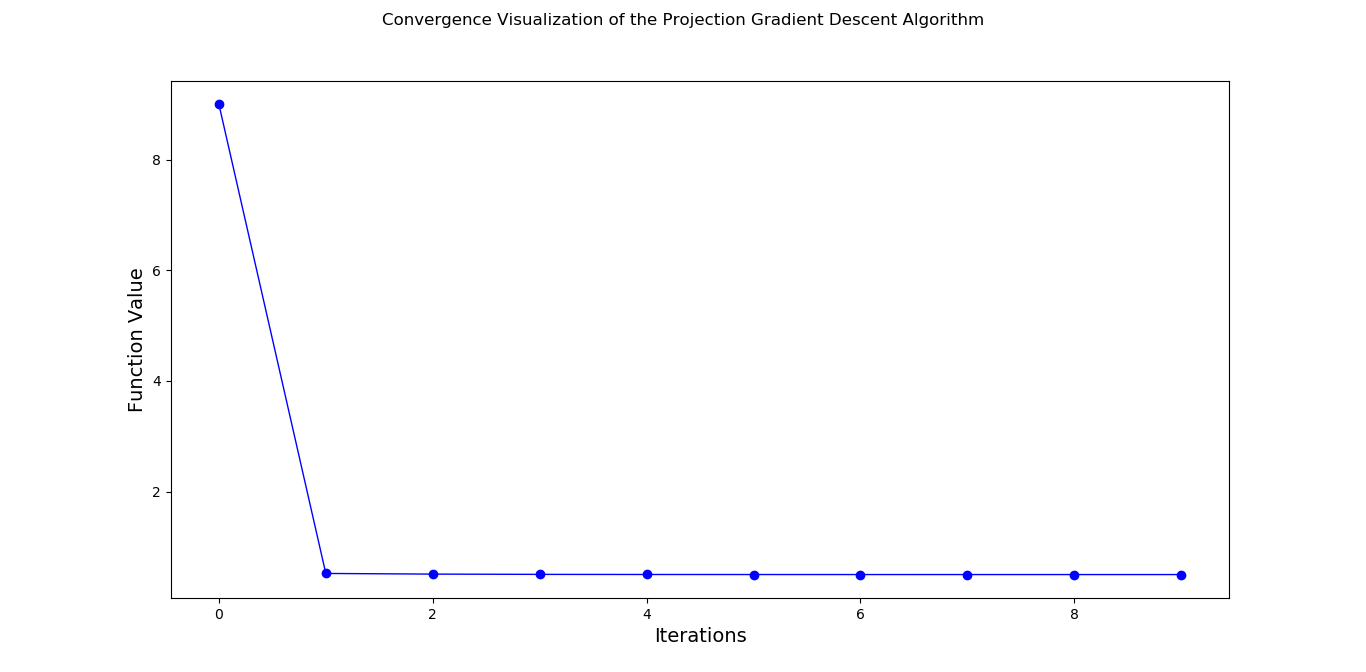
\includegraphics[width=1.0\textwidth]{PGD_Convergence_Gamma_Optimal_Point1.png}
\caption{Convergence Visualization of the Projection Gradient Descent Algorithm with step size $0.1$}
\label{fig:mesh7}
\centering
\end{figure}
$\gamma\ =\ 0.1$ [Figures (\ref{fig:mesh1}) and (\ref{fig:mesh7}) with different orders of magnitude along the x-axis] appears to be the best choice for the step size given the fact that it achieves convergence in one step.
\clearpage
\section{Optimal Power and Bandwidth Allocation}
\subsection{Problem Formulation}
\[maximize_{\vec{P},\ \vec{W}}\ \sum_{i=1}^n\ \alpha_i W_i log_2(1 + \frac{\beta_i P_i}{W_i})\]
\[subject\ to\ \sum_{i=1}^n\ P_i \leq P_{max},\ \sum_{i=1}^n\ W_i \leq W_{max},\ P_i \geq 0,\ and\ W_i \geq 0,\ \forall i\]
where, $P_{max} \geq 0$ and $W_{max} \geq 0$
Re-writing to turn it into a conventional minimization problem,
\[minimize_{\vec{P},\ \vec{W}}\ -\sum_{i=1}^n\ \alpha_i W_i log_2(1 + \frac{\beta_i P_i}{W_i})\]
\[subject\ to\ \sum_{i=1}^n\ P_i \leq P_{max},\ \sum_{i=1}^n\ W_i \leq W_{max},\ P_i \geq 0,\ and\ W_i \geq 0,\ \forall i\]
\\The problem formulated above is a convex optimization problem because,
\begin{itemize}
    \item $-log_2(1 + \frac{\beta_i P_i}{W_i})$ is a convex function because the projection of a convex function is also convex.
    \\If $f(x)$ is convex, $tf(\frac{x}{t})$ is also convex.
    \\Since we know that $log(1 + \beta_i P_i)$ is convex, the projection of this given by $W_i log(1 + \frac{\beta_i P_i}{W_i})$ is convex.
    \\Now, $\sum_{i=1}^n\ \alpha_i\ (-log_2(1 + \frac{\beta_i P_i}{W_i}))$ is convex because it is a non-negative weighted sum of convex functions.
    \\\textbf{So, the objective function is convex}.
    \item The feasible set is the intersection of a finite number of halfspaces, i.e. a polyhedron, which is a convex set.
    \\Therefore, \textbf{the feasible set is a convex set}.
\end{itemize}
\subsection{The Lagrangian and the Dual}
The Lagrangian is formulated as shown below,
\[\mathcal{L}(\vec{P},\ \vec{W},\ \lambda,\ \nu)\ =\ -\sum_{i=1}^n\ \alpha_i W_i log_2(1 + \frac{\beta_i P_i}{W_i}) + \lambda(\sum_{i=1}^n P_i - P_{max}) + \nu(\sum_{i=1}^n W_i - W_{max})\]
\[\frac{\partial \mathcal{L}}{\partial P_i}\ =\ 0\]
\[-\alpha_i W_i \frac{\frac{\beta_i}{W_i}}{1 + \frac{\beta_i P_i}{W_i}} + \lambda\ =\ 0\]
\[P_i\ =\ \frac{W_i}{\beta_i}(\frac{\alpha_i \beta_i}{\lambda} - 1)\]
If $\alpha_i \beta_i$ < $\lambda$, $P_i$ would become negative which would violate the $P_i \geq 0,\ \forall i$ constraint. 
\\Therefore, we use projection to project it back to $[0,\ P_{max}]$.
\[P_i\ =\ \frac{W_i}{\beta_i}\Big[\frac{\alpha_i \beta_i}{\lambda} - 1\Big]^+\]
For receivers with $\alpha_i \beta_i > \lambda$, using this result in the following sequence of steps,
\[\frac{\partial \mathcal{L}}{\partial W_i}\ =\ 0\]
\[\alpha_i\Big(\frac{-\beta_i P_i}{W_i} \frac{1}{(1 + \frac{\beta_i P_i}{W_i})ln 2} + \frac{ln(1 + \frac{\beta_i P_i}{W_i})}{ln 2}\Big) + \nu\ =\ 0\]
\[(ln 2)\nu\ =\ \alpha_i ln(\frac{\alpha_i \beta_i}{\lambda}) + \frac{\lambda}{\beta_i} - \alpha_i\]
We know that,
\[g(\lambda,\ \nu)\ =\ minimize_{\vec{P},\ \vec{W}}\ \mathcal{L}(\vec{P},\ \vec{W},\ \lambda,\ \nu)\]
\[\lambda^*,\ \nu^*\ =\ argmax_{\lambda,\ \nu}\ g(\lambda,\ \nu)\]
By maximizing the dual, we obtain the result that,
\\For all receivers $i \in \{1,\ 2,\ ....,\ n\}$ with $\alpha_i \beta_i > \lambda$, non-zero bandwidth is allocated if,
\[i\ =\ argmax_{i \in \mathcal{J}}\ \Big(\alpha_i ln(\frac{\alpha_i \beta_i}{\lambda}) + \frac{\lambda}{\beta_i} - \alpha_i\Big)\]
where,
\[\mathcal{J}\ =\ \{i:\ \alpha_i \beta_i > \lambda\}\]
\setstcolor{red}
\subsection{Sub-Gradient Projection in the Dual}
To update $\lambda$, we use the following update step,
\[\lambda_{k+1}\ =\ \Big[\lambda_k + \gamma \Big(\sum_{i=1}^n P_i - P_{max}\Big)\Big]^+\]
We iteratively update $\lambda$ along with updates to $W_i$ and $P_i$ using this updated value of $\lambda$ until $\lambda$ converges.
\\More specifically, after evaluating $\lambda_k$, for receivers having $\alpha_i \beta_i > \lambda_k$, we find the receiver maximizing $\alpha_i ln(\frac{\alpha_i \beta_i}{\lambda_k}) + \frac{\lambda_k}{\beta_i} - \alpha_i$. We assign all the bandwidth to this receiver. If multiple receivers turn out to be the maximizers, the available bandwidth is equally divided among them. Using these $W_i$ values, we update $P_i\ =\ \frac{W_i}{\beta_i}\Big(\frac{\alpha_i \beta_i}{\lambda} - 1\Big)$. We then calculate the sub-gradient as $\sum_{i=1}^n P_i - P_{max}$. Then, we calculate $\lambda_{k+1}\ =\ \Big[\lambda_k + \gamma \Big(\sum_{i=1}^n P_i - P_{max}\Big)\Big]^+$, the projection being into $[0, \infty)$. This sequence of steps is performed until $\lambda^{*}\ =\ \Big[\lambda^{*} + \gamma \Big(\sum_{i=1}^n P_i - P_{max}\Big)\Big]^+$, i.e. there are no further changes to $\lambda$ with respect to the projection gradient update indicating convergence.
\\Please refer to the source code (\textit{OptimalPowerAndBandwidthAllocation.py}) for further details.
\subsection{Simulation: Results}
\begin{figure}[t]
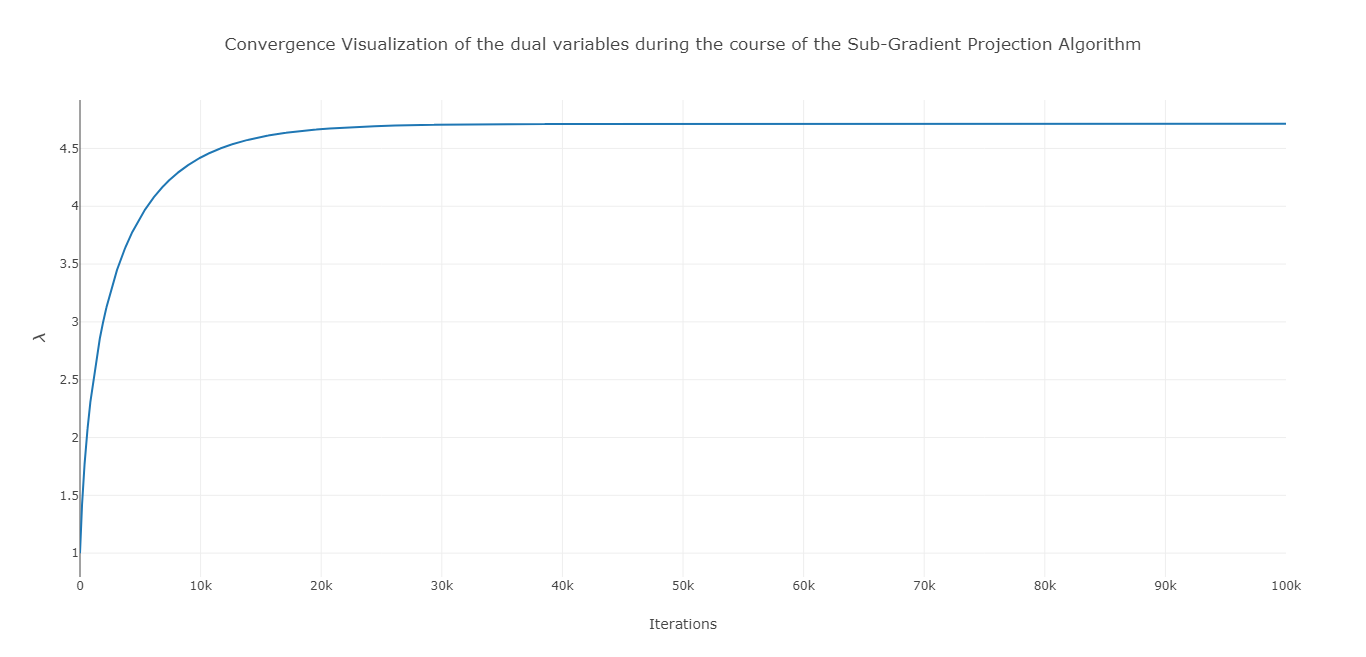
\includegraphics[width=1.0\textwidth]{Convergence_Plot_Step_Size_point001.png}
\caption{Convergence Visualization of the Sub-Gradient Projection Algorithm in the Dual with step size $0.001$}
\label{fig:mesh8}
\centering
\end{figure}
\begin{figure}[t]
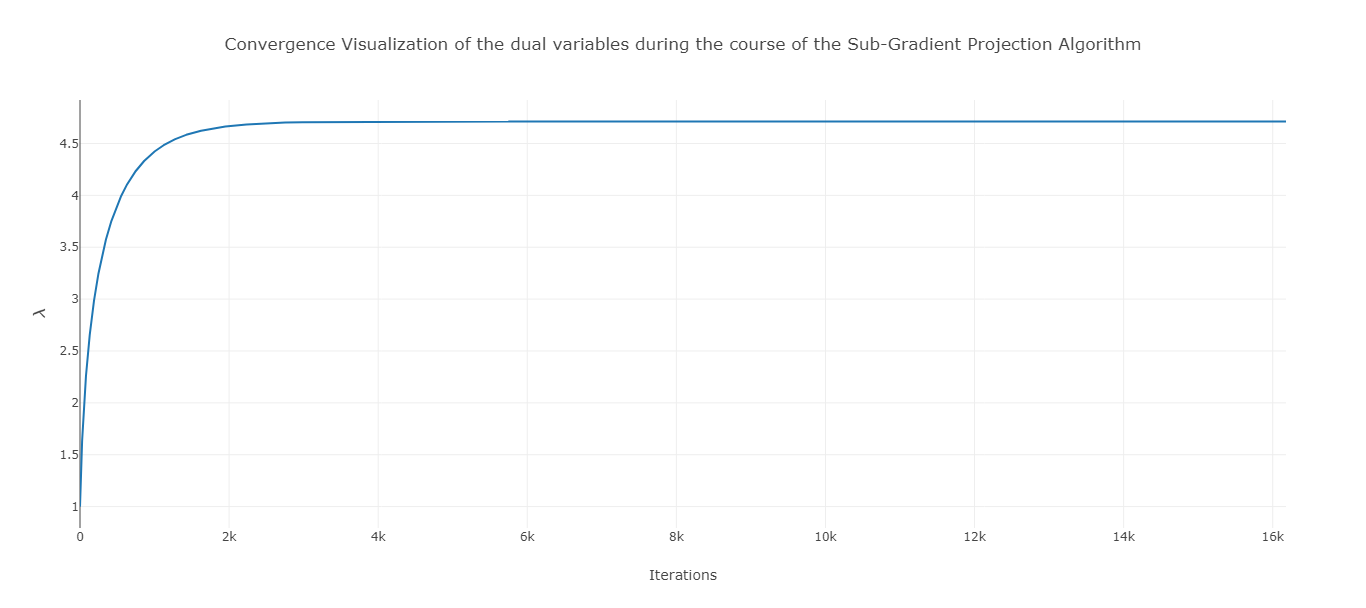
\includegraphics[width=1.0\textwidth]{Convergence_Plot_Step_Size_point01.png}
\caption{Convergence Visualization of the Sub-Gradient Projection Algorithm in the Dual with step size $0.01$}
\label{fig:mesh9}
\centering
\end{figure}
\begin{figure}[t]
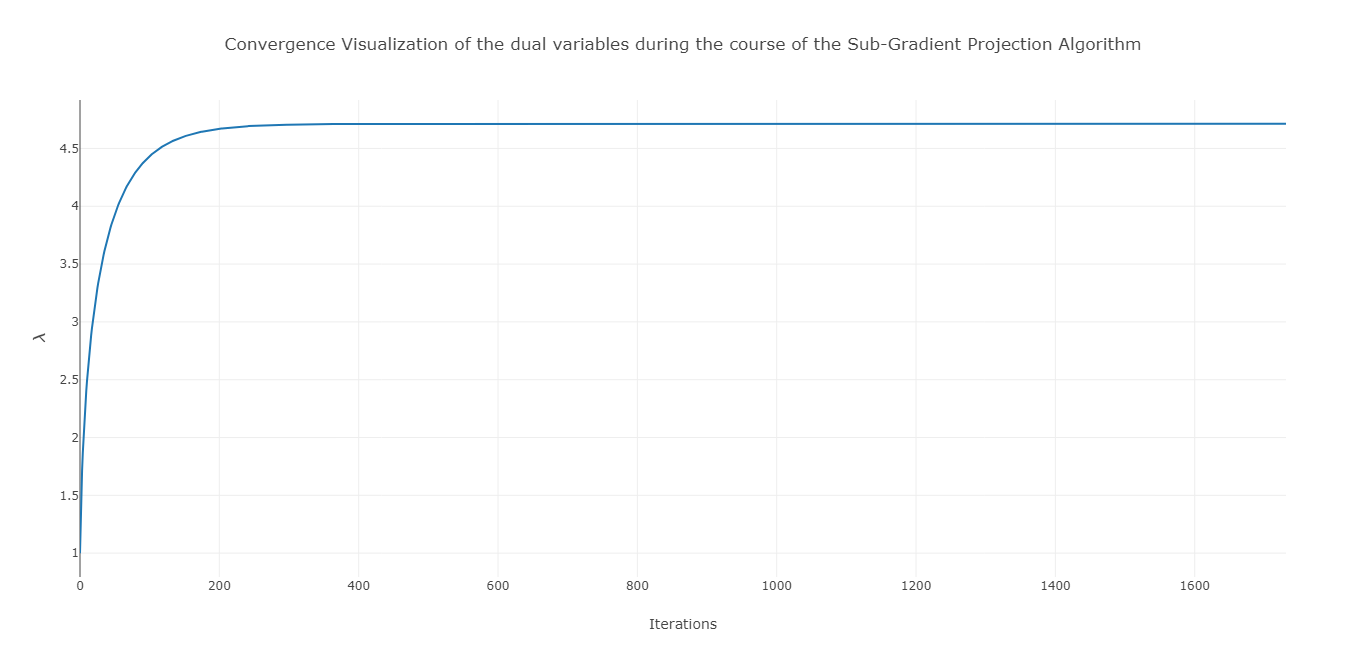
\includegraphics[width=1.0\textwidth]{Convergence_Plot_Step_Size_point1.png}
\caption{Convergence Visualization of the Sub-Gradient Projection Algorithm in the Dual with step size $0.1$}
\label{fig:mesh10}
\centering
\end{figure}
\begin{figure}[t]
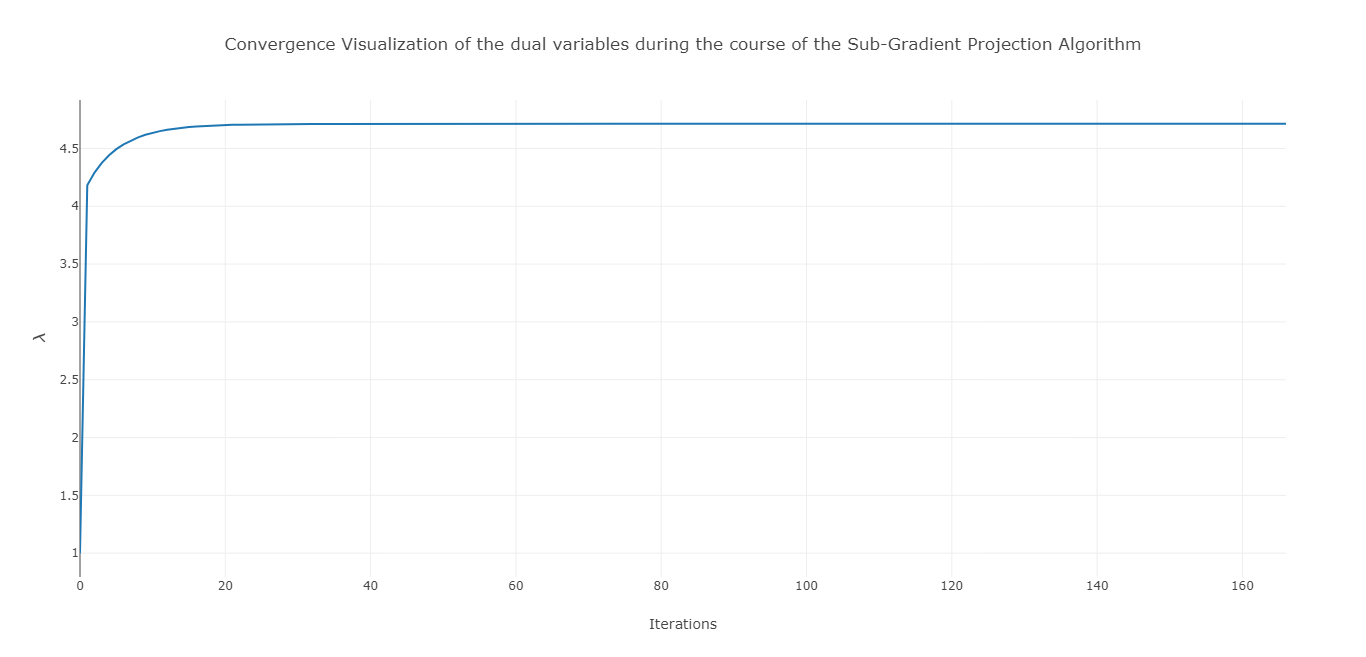
\includegraphics[width=1.0\textwidth]{Convergence_Plot_Step_Size_1.png}
\caption{Convergence Visualization of the Sub-Gradient Projection Algorithm in the Dual with step size $1$}
\label{fig:mesh11}
\centering
\end{figure}
\begin{figure}[t]
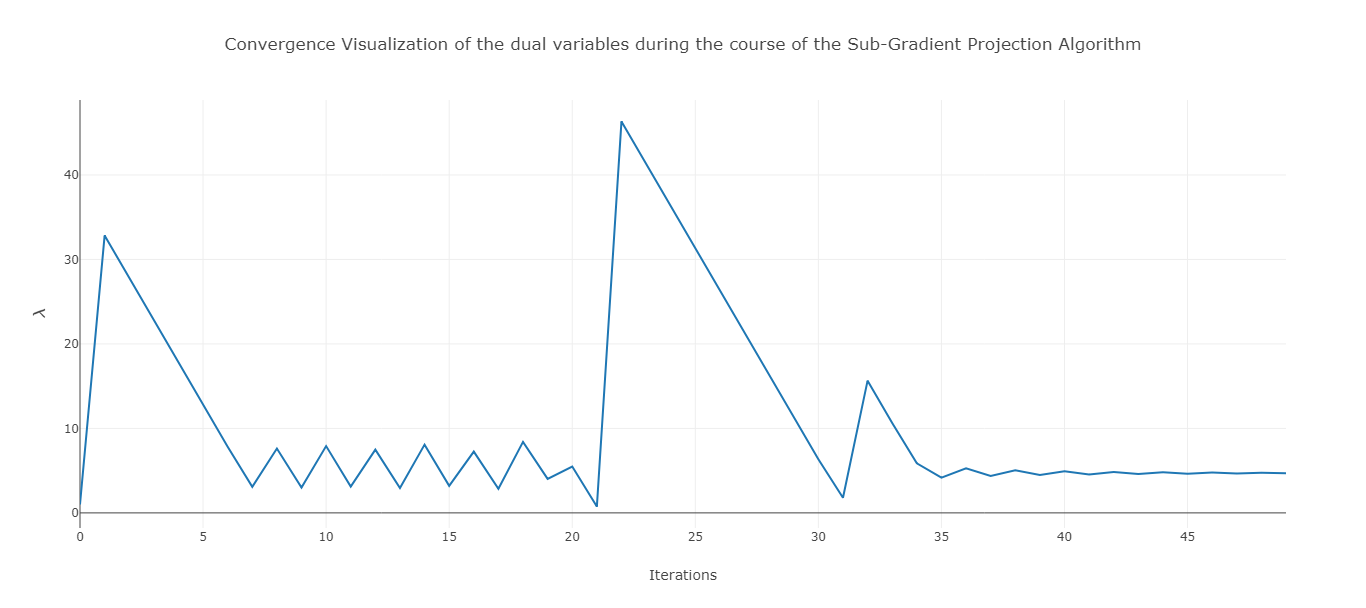
\includegraphics[width=1.0\textwidth]{Convergence_Plot_Step_Size_10.png}
\caption{Convergence Visualization of the Sub-Gradient Projection Algorithm in the Dual with step size $10$}
\label{fig:mesh12}
\centering
\end{figure}
\begin{figure}[t]
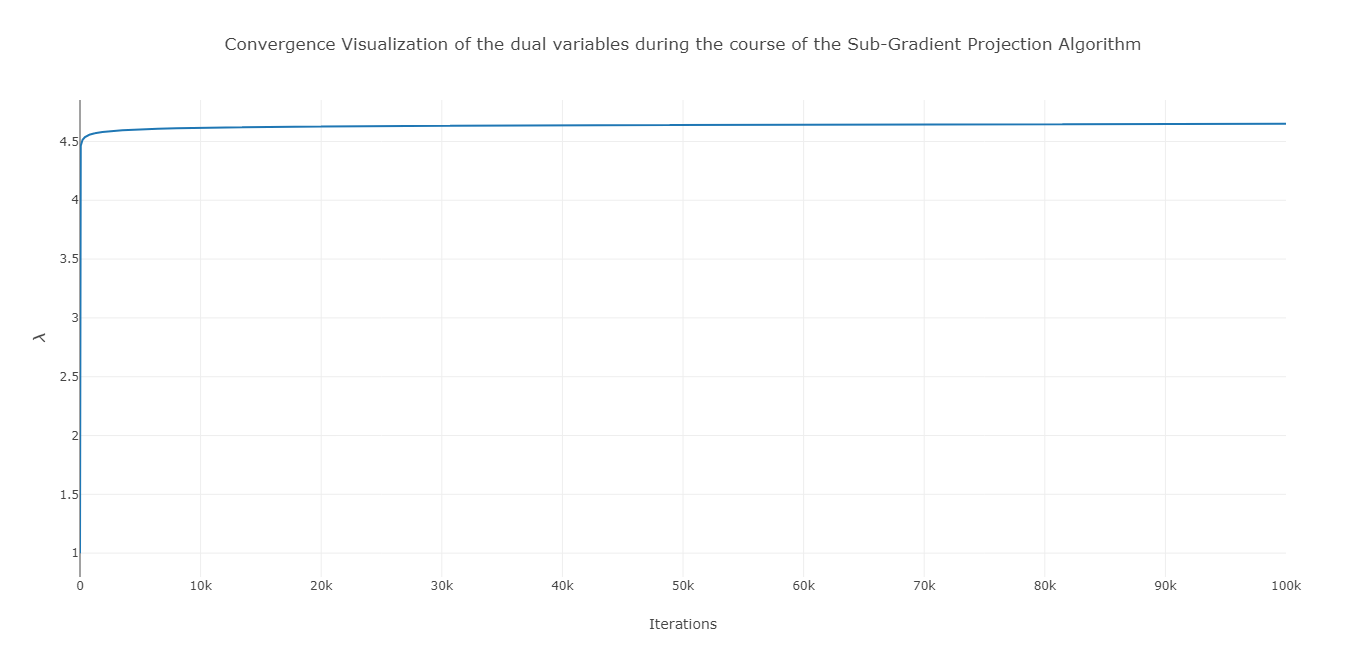
\includegraphics[width=1.0\textwidth]{Convergence_Plot_Step_Size_1byk_2.png}
\caption{Convergence Visualization of the Sub-Gradient Projection Algorithm in the Dual with step size $1/iteration\_count$}
\label{fig:mesh13}
\centering
\end{figure}
\clearpage
\subsubsection{Equal Power and Equal Bandwidth allocation strategy}
All users will get $\frac{P_{max}}{n}$ power allocation and $\frac{W_{max}}{n}$ bandwidth allocation leading to equal rates irrespective of $\alpha_i$ and $\beta_i$.
\subsubsection{Equal Bandwidth but Optimal Power Allocation}
All users/receivers are allocated equal bandwidth $\frac{W_{max}}{n}$ but, the power allocation is given by the water filling strategy.
\[P_i\ =\ \frac{W_i}{\beta_i}\Big[\frac{\alpha_i \beta_i}{\lambda} - 1\Big]^+\]
\end{document}